% -*- mode: LaTeX; fill-column: 100; -*-
% Local Variables for Emacs 
% M-q will fill current paragraph (fill-paragraph). 

\documentclass[acmtoms]{acmsmall}

\usepackage{amsmath}
\usepackage{amsfonts}
\usepackage{amssymb}
\usepackage{graphicx}
\usepackage{url} 
\usepackage{color}
\usepackage[ruled,vlined]{algorithm2e}
\usepackage{subfig}
\usepackage[hidelinks]{hyperref}
        
%% Our definition
\def\K{\mathbb{K}}
\def\N{\mathbb{N}}
\def\Z{\mathbb{Z}}
\def\F{\mathbb{F}}
\def\M{\mathsf{M}}
\def\C{\mathsf{C}}
\def\I{\mathsf{I}}
\def\R{\mathsf{R}}
\def\Q{\mathbb{Q}}

\def\Mat{\mathcal{M}}
\def\bigO{{\ensuremath{\mathcal{O}}}}

%\def\bigO{{\ensuremath{\operatorname{O}}}} 
%\def\bigO{{\ensuremath{\mathcal{O}}}}
%\markboth{}{}

%% TeXmacs macros
\newcommand{\tmop}[1]{\ensuremath{\operatorname{#1}}}
\newcommand{\assign}{:=}
\newcommand{\rem}{\tmop{rem}}
\newcommand{\quo}{\tmop{quo}}
\newcommand{\todo}[1]{(\textbf{todo:} #1)}


\title{
Simultaneous conversions with the Residue Number System using linear algebra
}
            
\author{
Javad Doliskani \affil{University of Waterloo}
Pascal Giorgi \affil{LIRMM CNRS - University of Montpellier}
Romain Lebreton \affil{LIRMM CNRS - University of Montpellier}
Eric Schost \affil{University of Waterloo}
}
           
\begin{abstract}
	We present an algorithm for simultaneous conversion between a given set of integers and their 
	Residue Number System representations based on linear algebra. We provide a highly optimized 
	implementation of the algorithm that exploits the computational features of modern processors. 
	The main application of our algorithm is matrix multiplication over integers. Our speed-up of 
	the conversions to and from the residue number system significantly improves the overall 
	running time of matrix multiplication. 
\end{abstract}
      
\category{G.4}{Mathematical Software}{Algorithm design and analysis} 
\category{F.2.1}{Analysis of Algorithms and Problem Complexity}{Numerical Algorithms and Problems}[computations in finite fields.]
\terms{Algorithms, Experimentation, Performance.}
\keywords{}
            
\begin{document}
            
            
\maketitle

%%%%%%%%%%%%%%%%%%%%%%%%%%%%%%%%%%%%%%%%%%%%%%%%%%%%%%%%%%%%
%%%%%%%%%%%%%%%%%%%%%%%%%%%%%%%%%%%%%%%%%%%%%%%%%%%%%%%%%%%%
%%%%%%%%%%%%%%%%%%%%%%%%%%%%%%%%%%%%%%%%%%%%%%%%%%%%%%%%%%%%

\section{Introduction}

There currently exist a variety of high-performance libraries for linear algebra or polynomial
transforms using floating point arithmetic~\cite{Whaley2001,Goto2008,FFTW05,Pueschel:05}.
High-performance kernels for linear algebra or polynomial arithmetic are also available in the
context of computations over the integers or finite fields, through libraries or systems such as
NTL~\cite{Shoup95}, FLINT~\cite{Hart2010}, FFLAS-FPACK~\cite{fflas-ffpack} or Magma~\cite{BoCaPl97}.

In this paper, we are interested in the latter kind of computation, in the context of multiple
precision arithmetic: we work with matrices or polynomials with coefficients that are
multi-precision integers, or lie in a finite ring $\Z/N\Z$, for some large $N$, and we consider a
basic operation such as the multiplication of these matrices or polynomials. There exist multiple
applications to this fundamental operation; we illustrate this in the last section of this paper
with a discussion of polynomial factorization.

To perform a matrix or polynomial multiplication in such a context, several possibilities exist. A
first approach consists in applying known algorithms, such as Strassen's, Karatsuba's, \dots
directly over our coefficient ring, relying {\it in fine} on fast algorithms for multiplication of
multi-precision integers. Another large class of algorithms relies on {\em modular techniques}, or
{\em residue number systems}, computing the required result modulo many small primes before
recovering the output by Chinese Remaindering.  One should not expect either of these approaches to
be superior in all circumstances. For instance, in extreme cases such as the product of matrices of
size $1$ or $2$ with large integer entries, the modular approach highlighted above is most likely
not competitive with a direct implementation. On the other hand, for the product of larger matrices
or polynomials, residue number systems often perform better than direct implementations, and as
such, they are used in libraries or systems such as NTL, FFLAS-FFPACK, Magma, \dots

In this paper, we present new techniques for residue number systems that are applicable in a wide
range of situations. In many cases, the bottlenecks in such an approach is the reduction of the
inputs modulo many small primes, and the reconstruction of the output from its modular images by
means of Chinese Remaindering; by contrast, operations modulo the small primes are often quite
efficient.

Algorithms of quasi-linear complexity have been known for long for both modular reduction and
Chinese Remaindering~\cite[Chapter~10]{GaGe13}, based on so-called subproduct tree techniques;
however, their practical performance remains somewhat lagging. Our algorithm offers an alternative
to this approach, for those cases where we have several coefficients to convert; it relies on
matrix multiplication to perform these tasks, with matrices that are integer analogues of
Vandermonde matrices and their inverses. As a result, while its complexity is inferior to that of
asymptotically fast methods, our algorithm behaves extremely well in practice, as it allows us to
rely on high-performance libraries for matrix multiplication.

\todo{Outline of the paper, acknowledgements.}

%%%%%%%%%%%%%%%%%%%%%%%%%%%%%%%%%%%%%%%%%%%%%%%%%%%%%%%%%%%%
%%%%%%%%%%%%%%%%%%%%%%%%%%%%%%%%%%%%%%%%%%%%%%%%%%%%%%%%%%%%
%%%%%%%%%%%%%%%%%%%%%%%%%%%%%%%%%%%%%%%%%%%%%%%%%%%%%%%%%%%%

\section{Preliminaries and notation}

We denote resp. by $(a \rem b)$ and $(a \quo b)$ the remainder and quotient of the Euclidean
division of $a \in \mathbb{Z}$ by $b \in \N$, with $0 \leqslant (a \rem b) < b$; we extend the
notation $(a \rem b)$ to any rational $a=n/d \in \Q$ such that $\gcd (d,b) = 1$ to be the unique
$\alpha$ in $\{0,\dots,b-1\}$ such that $\alpha d = n \bmod b$. We call informally a {\em
  pseudo-reduction} of $a$ modulo $p$ the computation of $b$ such that $a = b \bmod p$ and $b$ ``not
too big" compared to $p$. In practice, we often will have that $b =O (p^2)$.


We shall follow a bit complexity model in this paper, in the sense that our complexity statements
are given in terms of number of bit operations. In some cases, such as polynomial multiplication, it
is more convenient to state the complexity based on the number of operations in the coefficient
field.  These complexity statements remain the same in the bit complexity model when the coefficient
field has a constant element's size, i.e. a constant number of machine words.

% A classic way to represent a positive integer is to use a positional number system, with base
% $\beta$. Any integer $a \in \N$ can be uniquely written as $a = \sum_{i=0}^{n-1} a_i\beta^i$ for
% some $0 \leq a_i < \beta$, and $a$ is encoded as the vector $(a_{n-1},\hdots,a_1,a_0)$. One
% advantage of such a representation is that it allows us to represent arbitrary many integers, and
% compare or add integers in linear time in the number of digits. However, multiplication in this
% representation is more complex and requires quadratic time on the number of digits (better
% algorithms switch to another representation). Many other number systems provide better complexity
% for multiplication, but most of them loose the benefit of representing arbitrary many integers. In
% this article, we do not intend to present all different representations, and refer the reader to
% \cite{BrZi10,Bernstein08} for a survey on fast integer arithmetic. Instead, we only present the
% multi-modular representation that allows linear complexity for addition and multiplication of
% integers.
  
We let $\I(n)$ be such that two integers $a,b$ of sizes $|a|,|b| < 2^n$ can be multiplied in $\I(n)$
bit operations, assuming the base-2 expansions of $a$ and $b$ are given as input. The best known
bound for $\I(n)$ is $n\log(n)2^{O(\log^*(n))}$ uses Fast Fourier Transform and is due to
F\"urer~\cite{Furer07} (see~\cite{xxx,yyy} for further refinments). The arithmetic complexity of
multiplying two polynomials $f,g$ of degrees $\deg(f), \deg(g) \le n$ is denoted by $\M(n)$. This
means given a field $K$ and polynomials $f, g$ of degree $n$ over $K$, $fg$ can be computed in
$\M(n)$ arithmetic operations in $K$. The best known bound for $\M(n)$ is $O(n\log(n)\log\log(n))$
again using Fast Fourier Transform \cite{Schonhage1971,CaKa91}.  We assume that $\I$ and $\M$
satisfy the super-linearity assumptions of~\cite[Chapter~8]{GaGe13}.



%Should we take $\beta$ (\emph{e.g.} $2^{32}$ or $2^{64}$) as a constant and simplify complexity ?
%Yes and no : we will give complexities in
%$O( \dots\I(\log \beta) )$ and then specify that the term $\I(\log \beta))$
%can be removed when $\beta$ is a constant.



% For the sake of simplicity, we only consider operations on square matrices, and denote by
% $O(n^\omega)$ the upper-bound complexity of multiplying two matrices of dimension $n$.
**Notation $\M\M(r,s)$ **

% \paragraph{Organization of the paper}
% We first give an overview of the residue number system in Section \ref{sec:rns-overview}. In Section
% \ref{sec:ConvRNS}, we discuss algorithms for converting an integer to its Residue Number System
% representation, and vice versa. In Section \ref{sec:simul-rns}, we show how this conversion can be
% done simultaneously for a given set of integers. We then use these results to implement an efficient
% integer matrix multiplication algorithm in Sections \ref{sec:multi-mod-mm}, \ref{sec:impl}. Finally,
% we give sample applications of our results in Section~\ref{sec:exapp}.

%Say that our complexity model is bit complexity.
%
%
%Only give costs for the typical case $p_i \simeq \beta, s \simeq B, r
%\gg s$ because of $\beta^B < p_1 \cdots p_s$, which implies that $B < s$ ?
%
%Assume that $n \leqslant \beta$ !  Indeed we can assume that
%we won't have integers of more than $\beta$ machine words since it
%is the typical memory limit for a system whose address are encoded
%on a single precision integer. 
%
%We make this restriction to ensure the number of primes $s$
%necessary to encode the product of two $N \times N$ matrices of
%integers of size $n$ is still $\Theta(n)$ (the equation is
%$N \beta^{2n} \leqslant \beta^s$).

%%%%%%%%%%%%%%%%%%%%%%%%%%%%%%%%%%%%%%%%%%%%%%%%%%%%%%%%%%%%
%%%%%%%%%%%%%%%%%%%%%%%%%%%%%%%%%%%%%%%%%%%%%%%%%%%%%%%%%%%%
%%%%%%%%%%%%%%%%%%%%%%%%%%%%%%%%%%%%%%%%%%%%%%%%%%%%%%%%%%%%

\section{The Residue Number System}
\label{sec:rns-overview}

 
The Residue Number System (RNS) is a non-positional number system that allows us to represent a
finite subset of integers.  Let $m_1, m_2, \dots, m_s \in \N$ be pairwise coprime integers, and let
$M = m_1\times m_2 \times \hdots \times m_s$. Then any integer $a \in [0,\hdots,M-1]$ can be
uniquely determined by its residues $( [a]_{m_1}, [a]_{m_2}, \dots, [a]_{m_s})$. The uniqueness of
this residual representation is ensured by the the ring isomorphism
\begin{equation}\label{eq:crt} 
	\Z/M\Z \simeq \Z/m_1\Z \times \cdots \times \Z/m_s\Z.
\end{equation} 
This isomorphism is often called the Chinese Remainder Theorem (CRT) \cite[Section 5.4]{GaGe03}, and
this residual representation is called the Residue Number System. Assume the $m_i$ are fixed, and
denote $[a]_{m_i}$ by $[a]_i$ so that $([a]_1,[a]_2,\dots,[a]_s)_{\text{RNS}}$ is the representation
of the integer $a \in \N$.

In the RNS we can perform addition and multiplication independently on each residual.  Let
$a,b,c,d \in \N$ such that $c\equiv a + b \bmod M$ and $d \equiv a \times b \bmod M$ then
\begin{eqnarray}
	\label{addrns}
	([c]_1,[c]_2,\dots,[c]_s)_{\text{RNS}} &=& ([a]_1+[b]_1 \bmod m_1,\dots, [a]_s+[b]_s \bmod
	m_s)_{\text{RNS}}\\
	\label{mulrns}
	([d]_1,[d]_2,\dots,[d]_s)_{\text{RNS}} &=& ([a]_1\times 
	[b]_1 \bmod m_1,\dots, [a]_s\times [b]_s \bmod m_s)_{\text{RNS}} 
\end{eqnarray}
It is obvious from equations \ref{addrns} and \ref{mulrns} that addition and
multiplication in RNS require $O(s)$ operations on the residuals. One may
note that division in RNS is possible in the same way (individually on each
residual) only when the division is exact.

In order to benefit from RNS representation, one often need to convert back and
forth between the classic positional number system and RNS. Of course, these
conversions are costly and must be avoided when possible. However, when the
number of operations in RNS is high enough, these conversions can be neglected
and the RNS approach yields the most efficient solution.



%////////////////////////////////////////////////



\section{Converting one integer between classical and residue number systems}
\label{sec:ConvRNS}

In this section, we give an overview of two approaches for converting integers between classical and
residue number systems: the naive approach, and the quasi-linear approach.

\medskip
%%%%%%% TO BE INTEGRATED - ESPECIALLY 1 AND 4 WHICH WILL BE REQUIRED LATER
**Cost of both rem and quo to have cost of exact division**

We will recall in this paragraph the cost of computing $a \rem p$
together with $a \quo p$ for various sizes of $a$ and $p$. First, we can suppose w.l.o.g. that
$a \le 0$ and $a \le p$. Let $a \in\Z$ and $p \in \N$ such that $|a|<2^n$ and $p<2^m$.

\begin{enumerate}
  \item $n = \Theta (m)$.  Algo of \cite{Barrett86,Montgomery85} when $0 \le a < \beta^2$, $ \beta/2 < p < \beta$ for some $\beta$ (typically $\beta$ is a power of two) \cite{BrZi10}[Section 2.4.1]. Cost $O(\I(\log \beta))$.
    -- 
    \begin{equation}\label{eq:complexityReduction1} 
      O \left( \I (m) \right)
    \end{equation}
  
  \item $n \gg \Theta (m)$ Is established in 3.1 - Algorithm 1. Mentionned in \cite{BrZi10}[Section 2.4.1]
    \begin{equation}\label{eq:complexityReduction2} 
      O \left( \frac{n}{m} \I(m) \right)
    \end{equation}
  
  \item $n-m \ll \Theta (m)$ Will be useful to finish the Euclidean division when we have a pseudo-reduction. One reference could be \cite{GII13}[Algorithm 2].
  
  \begin{equation}\label{eq:complexityReduction3} 
    O \left( \I (n-m) \frac{m}{n-m} \right)
  \end{equation}

  \item Fast version of \ref{eq:complexityReduction2}. Established in 3.2. $C(s) = O( \frac{\I(n/m) \log (n/m)}{n/m} \I(\log m))$ ??.
\end{enumerate}


% \subsection{Naive approach}
% \label{sssec:naivetoRNS}

% \paragraph{Conversion to RNS} In order to convert an integer $a$ to its representation in the
% residue number system $(m_1, \cdots, m_s)$, one can simply compute of $a \bmod m_i$ for
% $i\in \{1,\hdots,k\}$ using the Euclidean division. Let us assume the particular case
% $m_1,\dots,m_s<\beta$ and $a<\beta^n$, where $\beta$ is bound by a certain number of machine words.
% In fact, this case represents computation on finite machines that are used in practice.

% \vspace*{2mm}
% \begin{algorithm}[H]
% \DontPrintSemicolon
% 	\KwIn{$a=\sum_{i=0}^{n-1}a_i\beta^i, m_j \in \N$}
% 	\KwOut{$a \bmod m_j$} 
% 	$c=a_{n-1}$\\
% 	\lFor{$i=n-2$ \textbf{to} $0$}
% 	{ 
% 	  $c = c \beta + a_i \bmod m_j$ \hfill // Use Barrett's algorithm
% 	} 
% 	\Return{$c \bmod m_j$}\;
% 	\caption{Modular reduction}
% \end{algorithm}
% \vspace*{2mm}

% The bit complexity for computing $a \bmod m_j$ is $O(n \I(\log \beta))$.
% Therefore, conversion to RNS costs $O(sn\I(\log \beta))$ bit operations.
% When $\beta$ is a constant, e.g. as large as a few machine words, the cost
% becomes $O(sn)$.

% The case when the $m_j$'s are almost of the same size as $a$,
% i.e. $m_1,\dots,m_s \in \beta^{\Theta(n)}$, is more classical and can be handled
% through integer multiplications using Barrett or Montgomery algorithms
% \cite{Barrett86,Montgomery85}. The cost of modular reduction then becomes
% $O(\I(n\log \beta))$ bit operations and conversion to RNS costs
% $O(s\I(n\log \beta))$.  This boils down to $O(s\I(n))$ when $\beta$ is
% fixed.

% \paragraph{Conversion from RNS}
% Let $a$ be an integer given by its RNS representation $([a]_1, \dots, [a]_s)$ with the base
% $(m_1,\dots,m_s)$. In order to retrieve the value of $a$ written in base $\beta$,
% i.e. $a=\sum_{i=0}^{n-1}a_i\beta^i$, one needs to solve the following system of congruences in the
% $a_i$:
% \begin{eqnarray}
%  \left[a\right]_1 &\equiv& \sum_{i=0}^{n-1}a_i\beta^i \bmod m_1\nonumber \\ 
%  & \vdots & \\ 
%  \left[a\right]_s & \equiv & \sum_{i=0}^{n-1}a_i\beta^i \bmod m_s \nonumber
% \end{eqnarray}
% A solution to this linear system is given by the Chinese Remainder Theorem recalled in Equation
% \ref{eq:crt}.  Let $M=\Pi_{i=1}^sm_i$ and $M_i=(M/m_i) \rem m_i$. The solution can be computed using
% the sum
% \begin{equation}\label{eq:cra}
% a \equiv \sum_{i=1}^s M_i ([a]_i / M_i \bmod m_i) \bmod M.
% \end{equation}
% Assume that $M$ and $M_i^{-1} \bmod m_i$ are precomputed for all $1 \le i \le s$. Then each
% multiplication $a'_i \assign ([a]_i / M_i \bmod m_i)$ costs $O(\I(\log \beta))$ and each unbalanced
% multiplication $M_i a'_i$ costs $O(s \I(\log \beta))$, since $M_i<\beta^s$ and $a'_i <
% \beta$. Finally, the sum is bounded
% \[
% \sum_{i=1}^s M_i a'_i < s\beta^s
% \]
% and its reduction cost is $O(s \log s \log \beta)$ (using formula \eqref{eq:complexityReduction3})
% which is not dominant. Therefore the total cost is $O(s^2\I(\log \beta))$ bit operations.

% For the precomputation, $M$ can be computed can be computed with $s$ unbalanced multiplications at a
% cost of $O(s^2 \I(\log \beta))$ bit operations. Then each unbalanced exact division $M/m_i$ is
% computed using $O(s \I(\log \beta))$ bit operations. The corresponding reduction modulo $m_i$ also
% costs $O( s \I(\log \beta))$ using formula \eqref{eq:complexityReduction2}. Finally, computing each
% $M_i^{-1} \bmod m_i$ cost $O(\I(\log \beta) \log \log \beta)$. Altogether, the precomputation
% costs $O( (s^2 + s \log \log \beta) \I(\log \beta))$ bit operations.

% \subsection{Quasi-linear approach}

% In this section, we briefly recall the quasi-linear algorithm based on binary multiplication tree to
% convert with the RNS due to \cite{Borodin1974}. We follow the exposition given in
% \cite{Borodin1974} and \cite{GaGe03}[Section 10.3].

% \paragraph{Conversion to RNS}
% The first step of the algorithm is a computation of the binary multiplication
% tree of the moduli $m_i$. Assume for the sake of simplicity that $s= 2^\kappa$.
% Starting from $m_1,\dots,m_s$, we compute the first level of the tree made of
% the products $m_1 m_2, m_3 m_4, \dots, m_{s-1} m_s$, then the second level made
% of the products $m_1 m_2 m_3 m_4, \dots, m_{s-3} \cdots m_s$ from the first level. And
% so on down to the last level of height $\kappa$ made of the full product
% $m_1 m_2 \cdots m_s$. The cost of computing this binary multiplication tree is
% $O(\I(s) \log s \I(\log \beta))$ when all the moduli are less than $\beta$.
% This boils down to $O(\I(s) \log s)$ when $\beta$ is a constant. 

% The second step of the algorithm is recursive and uses a divide-and-conquer
% approach. In order to reduce an integer $a$ modulo $m_1,\dots,m_s$, we compute
% $a_l = a \rem m_1 \cdots m_{s/2}$ and $a_h = a \rem m_{s/2+1} \cdots m_s$. We then recursively 
% reduce $a_l$ modulo $m_1,\dots,m_{s/2}$ and $a_h$ modulo $m_{s/2+1},\dots,m_s$, and we are
% done. Note that the products $m_1 \cdots m_{s/2}$ and $m_{s/2+1} \cdots m_s$
% were precomputed, and the same goes for the products required in all the recursive
% calls. The cost $C(s)$ of the reduction satisfies $C(s) = 2 C(s/2) + O(\I(s) \I(\log \beta))$ which 
% yields $C(s) = O( \I(s) \log s \I(\log \beta))$.

% \paragraph{Conversion from RNS}

% The backwards conversion is a bit trickier. It still follows Formula
% \eqref{eq:cra} together with a divide-and-conquer approach. The first step is to precompute 
% $M_i^{-1} \rem m_i$ for all $1 \leqslant i \leqslant s$ in time $O( \I(s) \log s \I(\log \beta))$. 
% For this, we use the above quasi-linear conversion to RNS to
% compute $M$ modulo $m_1^2,\dots,m_s^2$. Then we recover
% $M_i \rem m_i = \left(M \rem m_i^2 \right)/m_i$ with an exact integer
% division. It remains to compute the inverses of $(M_i \rem m_i)$ modulo $m_i$
% which amounts to $O(s \I(\log \beta))$ bit operations.

% Now let $s_i = \left([a_i] (M_i^{-1} \rem m_i)\right) \rem m_i$.  Formula
% \eqref{eq:cra} gives $a \equiv \sum_{i=1}^s s_i (M/m_i) \bmod M$ which is
% computed recursively as follows. Let $M_l \assign m_1 \cdots m_{s/2}$ and $M_h 
% \assign m_{s/2+1} \cdots m_s$. We first compute 
% \[
% \renewcommand{\arraystretch}{1.5}
% \begin{array}{lll}
% 	a_l & = & \sum_{i=1}^{s/2} s_i (M_l/m_i) \bmod M\\
% 	a_h & = & \sum_{i=s/2+1}^{s} s_i (M_h/m_i) \bmod M
% \end{array}
% \]
% recursively, and then recover $a$ using $a = M_h \cdot a_l + M_l \cdot a_h$.
% This recursive algorithm costs $C(s) = 2 C(s/2) + O(\I(s/2) \I(\log \beta))$
% which yields $C(s) = O( \I(s) \log s \I(\log \beta))$ as before.

\subsection{Summary of complexities}

In the following table, we recall all the complexities for conversions with RNS representation. We assume that the RNS basis is given as $(m_1,\dots,m_s)$ such that each $m_i<2^t$ and integers to
convert have $n$-bits with $n=\Theta(st)$.

\begin{table}[h]
\centering
\begin{tabular}{|l|r|r|}
\hline
               & conversion from RNS & conversion to RNS\\
\hline
naive approach & $\bigO(s^2\M(t))$ & $\bigO(s^2\M(t))$\\
fast approach  & $\bigO(\M(s)\log s~\M(t))$ & $\bigO(\M(s)\log s~\M(t))$ \\
\hline
\end{tabular}
\end{table}


%////////////////////////////////////////////////


\section{Simultaneous RNS conversions}
\label{sec:simul-rns}

The algorithms of Section \ref{sec:ConvRNS} enable us to convert back and forth between individual 
integers and their representations in a given residue number system. In this section, we discuss 
the problem of performing these conversions simultaneously between a given set of integers $a_1, 
\ldots, a_r \in \Z$ and their representations in a given residue number system $m_1, \ldots, m_s$. 
Assume for the entire section that $m_1, \ldots, m_s < \beta$ and $a_j < \beta^n$. 

\subsection{Direct approach}

The simplest approach is to apply the conversions of Section~\ref{sec:ConvRNS} to each $a_i$ 
separately. Of course, the precomputations of these algorithms are independent of the input 
integer. So, they are done once and for all. The complexity of simultaneous conversions is then
$O(rs^2 \I (\log \beta))$ for the naive approach, and $O(r \I (s) \log s \I(\log \beta))$ for the 
quasi-linear approach.

Note that, in term of implementation, simultaneous reductions using the naive
algorithms can benefit from vectorized (SIMD) instructions to lower the constant,
and can be easily parallelized. On the other hand, simultaneous reductions using
the quasi-linear approach do not benefit from SIMD instructions (or at least not
straightforwardly).

\subsection{Linear Algebra approach}

\paragraph{Conversion to RNS}
The conversion to RNS is split up to two phases: first we reduce the computation of 
pseudo-reductions of $a_i \bmod m_\ell $ to the reductions of $\beta^j \rem m_\ell$ for
$0 \leqslant j < n$ and $1 \leqslant \ell \leqslant s$ using one matrix
multiplication. Then we turn the pseudo-reductions into reductions in 
negligible time. We can precompute the values
$r_{j, \ell} \assign 2^{\beta j} \rem m_\ell$, which do not depend on the $a_i$, once and for all.  
The costs of the precomputation is $O( sn \I (\log (\beta)))$. It is done by incrementally 
computing the powers $\beta^j$ once, and then reducing them modulo the $m_\ell$. The simultaneous 
pseudo-reductions are done as follows. We first write the expansion in base $\beta$ of $a_i$:
\[ a_i = \sum_{j = 0}^{n - 1} c_{i,j} 2^{\beta j}, \qquad 1 \leqslant i \leqslant r. \] 
Let $a_{i, \ell} \assign \sum_{j = 0}^{n - 1} c_{i, j} r_{j, \ell}$ so that 
$a_{i, \ell} \equiv a_i \bmod m_{\ell}$. The value $a_{i, \ell} $ is bounded by
$n \beta^2$, since $a_i < \beta^n$ by assumption. We say that $a_{i, \ell}$ is a
pseudo-reduction of $a_i$ modulo $p_{\ell}$.
The values $a_{i, \ell}$ can be computed using linear algebra :
$(a_{i, \ell}) \in \Mat_{r \times s} (\Z)$ is the product of
$(c_{i, j}) \in \Mat_{r \times n} (\Z)$ and
$(r_{j, \ell}) \in \Mat_{n \times s} (\Z)$. If we write $a_{i, \ell} = [a_i]_{m_\ell}$, and $r_{j, 
\ell} = [2^{\beta j}]_{m_\ell}$ the pseudo-reduction is done using the following matrix 
multiplication.
\[
\renewcommand{\arraystretch}{1.5}
\begin{bmatrix}
	[a_1]_{m_1} & \cdots & [a_1]_{m_s} \\
	[a_2]_{m_1} & \cdots & [a_2]_{m_s} \\
	\vdots & \ddots & \vdots \\
	[a_r]_{m_1} & \cdots & [a_r]_{m_s} \\
\end{bmatrix}
=
\begin{bmatrix}
	c_{11} & c_{12} & \cdots & c_{1n} \\
	c_{21} & c_{22} & \cdots & c_{2n} \\
	\vdots & \vdots & \ddots & \vdots \\
	c_{r1} & c_{r2} & \cdots & c_{rn} \\
\end{bmatrix}
\times
\begin{bmatrix}
	1 & 1 & \cdots & 1 \\
	[2^\beta]_{m_1} & [2^\beta]_{m_2} & \cdots & [2^\beta]_{m_s} \\
	\vdots & \vdots & \ddots & \vdots \\
	[2^{\beta(n - 1)}]_{m_1} & [2^{\beta(n - 1)}]_{m_2} & \cdots & [2^{\beta(n - 1)}]_{m_s} \\
\end{bmatrix}
\]
This product costs $O( \M\M(r,n,s) \I(\log \beta))$ 
where $\M\M(,,)$ is the complexity of non-square matrix multiplication. In the most common
case we have $a_j < m_1 \cdots m_s$, which means $n = O(s)$. In that case, the above product can be 
split into $r / s$ products of square matrices of dimension $s$. The complexity then
reduces to $O(rs^{\omega - 1} \I (\log (\beta)))$. Now, the cost of computing the remainder
$(a \rem m)$, when $a < n \beta^2$ and $m < \beta$, is
$O \left( \I (\log (\beta)) \right)$. Therefore, our final step to compute the simultaneous 
reductions costs $O \left( r s \I (\log (\beta)) \right)$.

\paragraph{Conversion from RNS}
We perform \textit{simultaneous pseudo-reconstructions} as follows.
Recall that we denote $M=\Pi_{i=1}^sm_i$ and $M_i=(M/m_i) \rem m_i$ for
$1 \leqslant i \leqslant s$.  Let $l_i \assign \sum_{j = 1}^s a_{i, j} M_j [M_j^{- 1}]_{m_j}$ so 
that $a_i = l_i \bmod M$ (see Formula \eqref{eq:cra}) and $l_i < M \beta$. We say
that $l_i$ are pseudo-reconstructions of $(a_{i, \ell})$ modulo
$m_1, \ldots, m_s$. Let us precompute $M_{\ell} [M_{\ell}^{- 1}]_{m_{\ell}}$ for all
$1 \leqslant \ell \leqslant s$. If we have precomputed the $M_\ell$ before
(\emph{e.g.} during the reduction step), then we can compute
$[M_{\ell}]_{m_{\ell}}$ from $M_\ell$ in time $O(s \I(\log \beta))$, then
$[M_{\ell}^{-1}]_{m_{\ell}}$ in time $O(\I(\log \beta) \log \log \beta)$ and
finally $M_{\ell} [M_{\ell}^{- 1}]_{m_{\ell}}$ in time
$O(s \I(\log \beta))$. When $\beta$ is a constant, this comes down to
$O(s)$ bit operations. Now we write $M_{\ell} [M_{\ell}^{- 1}]_{m_{\ell}}$ in base $\beta$ as
\[
M_j [M_j^{- 1}]_{m_j} = \sum_{k = 0}^{s - 1} e_{j, k} \beta^k,
\]
and then we can write $l_i$ as
\[ 
l_i = \sum_{j = 1}^s a_{i, j} M_j [M_j^{- 1}]_{m_j} = \sum_{j = 1}^s
a_{i, j} \sum_{k = 0}^{s - 1} e_{j, k} \beta^k = \sum_{k = 0}^{s - 1} \left(
  \sum_{j = 1}^s a_{i, j} \cdot e_{j, k} \right) \beta^k . 
\]
The last inner sum can be computed using the following matrix multiplication
\[
\renewcommand{\arraystretch}{1.5}
\begin{bmatrix}
	d_{11} & d_{12} & \cdots & d_{1s} \\
	d_{21} & d_{22} & \cdots & d_{2s} \\
	\vdots & \vdots & \ddots & \vdots \\
	d_{r1} & d_{r2} & \cdots & d_{rs} \\
\end{bmatrix}
=
\begin{bmatrix}
	a_{11} & a_{12} & \cdots & a_{1s} \\
	a_{21} & a_{22} & \cdots & a_{2s} \\
	\vdots & \vdots & \ddots & \vdots \\
	a_{r1} & a_{r2} & \cdots & a_{rs} \\
\end{bmatrix}
\times
\begin{bmatrix}
	e_{11} & e_{12} & \cdots & e_{1s} \\
	e_{21} & e_{22} & \cdots & e_{2s} \\
	\vdots & \vdots & \ddots & \vdots \\
	e_{s1} & e_{r2} & \cdots & e_{ss} \\
\end{bmatrix}
\]
This product can be computed in $O \left( rs^{\omega - 1} \I (\log (\beta)) \right)$ bit 
operations. From the matrix $(d_{ij})$ we get $l_i = \sum_{k = 0}^{s - 1} d_{i, j} \beta^k$.
Note that $(d_{i, j})$ are not the exact coefficients of the $\beta$-expansion
of $l_i$. But we can still compute the $l_i$s in time $O(r s \I(\log \beta))$
since $d_{i, j} \leqslant s \beta^2$ and $s \leqslant \beta$ by assumption.
The final step of the reconstruction
consists in reducing $l_i$ modulo $M$. This step is relatively cheap since $l_i$
is almost reduced.  Using $s < \beta$ and $l_i =O (s \beta^{s + 2}) = O(\beta^{s + 2})$ and
$M =O (\beta^s)$, the last reduction step costs $O \left( s \I (\log \beta) \right)$ per $l_i$. 
Thus a total cost of $O (r s \I (\log \beta))$.


%////////////////////////////////////////////////


\section{Matrix multiplication with multi-precision integer entries}
\label{sec:multi-mod-mm}

In this section, we show how two matrices with multi-precision integer entries can be multiplied 
efficiently. The idea is to reduce to multiplication of matrices with small entries, which can then 
be performed using highly efficient architecture-aware algorithms. 

Let $A, B \in \Z^{n \times n}$ be integer matrices such that $\lVert AB \rVert_\infty < 2^k$, 
i.e. the entry size of the product is at most $k$ bits, for a positive integer $k$. Computing the 
product using the naive algorithm takes $O(n^\omega \I(k))$. This neither give the best complexity 
nor the best practical result as we will see later on. To compute $AB$ efficiently we proceed as 
follows. We first generate enough primes $m_1, m_2, \dots, m_s$ with $m_i < \beta$ such that 
$\lVert AB \rVert_\infty < M = m_1m_2 \cdots m_s$. The number $s$ of the primes is obviously 
bounded by $k$, so we have $s = O(k)$. Next, we compute $A_i = A \bmod m_i$ for all $1 
\le i \le s$, and similarly for $B_i$. This is done using the algorithms in Section 
\ref{sec:simul-rns}. Now the matrices $A_i, B_i$ have small entries, and the 
products $A_iB_i$ can be computed efficiently. Finally, we reconstruct $AB$ from $A_iB_i$ again 
using the algorithms in Section \ref{sec:simul-rns}. Algorithm \ref{algo:multi-m-m} summarizes this 
approach.

\vspace*{2mm}
\begin{algorithm}[H]
	\KwIn{$A, B$, and precomputed values related to $m_i$, $1 \le i \le k$}
	\KwOut{$AB$} 
	\For{$i=1$ to $k$}
	{ 
		$A_i \leftarrow A \bmod m_i$ \\
		$B_i \leftarrow B \bmod m_i$ \\
	} 
	\For{$i=1$ to $k$}
	{ 
		$C_i \leftarrow A_iB_i$ \\
	}
	Reconstruct $AB$ from $C_i$ \\
	\Return{$AB$}
	\caption{Multi-Modular matrix multiplication}
	\label{algo:multi-m-m}
\end{algorithm}
\vspace*{2mm}

Here, we do $O(k)$ matrix-matrix multiplications with small entries at the cost of $O(n^\omega k)$. 
Adding the costs of reduction and reconstruction, we get the final complexities of $O(n^\omega k + 
n^2k^2)$ for the naive RNS, $O(n^\omega k + n^2\I(k)\log(k))$ for quasi-linear RNS, and $O(n^\omega 
k + n^2k^{\omega - 1})$ for the linear algebra RNS. 

The above technique of reducing to matrices of small integers is not unique to the RNS approach. 
Other multi-precision integer multiplication approaches such as the ones in \cite{Schonhage1971} 
and \cite{Pollard1971} can be used, in much the same spirit. In \cite{Schonhage1971}, the input 
integer is recursively split into vectors of smaller chunks, and then FFT conversions are used to 
multiply those vectors. Adapting the algorithm to matrices, one requires $O(k \log(k))$ 
multiplications of matrices with small entries, and $n^2$ applications of FFT each costing $O(k 
\log(k)\log\log(k))$ operations. This gives the overall complexity of $O(n^\omega k + n^2k 
\log(k)\log\log(k))$ for multi-precision integer matrix multiplication.

To adapt the algorithm in \cite{Pollard1971} we consider matrices of polynomials $\mathcal{A}, 
\mathcal{B} \in \Z[X]^{n \times n}$ with the following conditions:
\begin{enumerate}
	\item $\lVert \mathcal{A}_{ij} \rVert, \lVert \mathcal{B}_{ij} \rVert < 2^\beta$, i.e. 
	polynomial entries have coefficients smaller than $2^\beta$.
	\item $\mathcal{A}(2^\beta) = A, \mathcal{B}(2^\beta) = B$, i.e. evaluating the polynomial 
	entries gives the input.
	\item $\deg(\mathcal{A}), \deg(\mathcal{B}) < d = O(k)$, i.e. polynomial entries have degrees 
	smaller than $d$.
\end{enumerate}
We also let $M = m_1m_2 \cdots m_t$ with primes $m_i < 2^{O(1)}$ such that $d2^{2\beta + \log n} < 
M < 2^{2\beta + \log n + \log k}$. Then $AB$ can be computed using $t$ products of polynomials 
matrices over $\Z[X] / m_i \Z[X]$ and CRT. This requires $d$ multiplications of matrices of small 
integers, and $n^2$ polynomial multiplications. The overall complexity is therefore $tO(n^\omega d 
+ n^2\M(d))$. We have $t = O(\log n + \log k)$. Since $d = O(k)$ and $d < m_i$ the complexity 
simplifies to $O(n^\omega kC + n^2 k\log k C)$ where $C = O(\log n + \log k)$. Table 
\ref{table:complexities} summarizes the asymptotic complexities of the mentioned matrix 
multiplication algorithms.
\begin{table}[h]
	\renewcommand{\arraystretch}{1.4}
	\tbl{Integer matrix multiplication complexities\label{table:complexities}}{
	\begin{tabular}{|l|ll|}
		\hline
		\multicolumn{1}{|c|}{\bf Algorithm} & \multicolumn{2}{c|}{\bf Complexity} \\
		\hline
		\hline
		Naive algorithm & $O(n^\omega \I(k))$ & \\
		Multi-modular + naive CRT & $O(n^\omega k$ & $+ n^2k^2)$ \\
		Multi-modular + fast CRT \cite{Borodin1974} & $O(n^\omega k$ & $+ n^2\I(k)\log(k))$ \\
		Kronecker + multi-mod FFT \cite{Pollard1971} & $O(n^\omega kC$ & $+ n^2 k\log(k)C)$ \\
		\cite{Schonhage1971} & $O(n^\omega k$ & $+ n^2k \log(k)\log\log(k))$ \\
		Multi-modular + linear algebra CRT & $O(n^\omega k$ & $+ n^2k^{\omega - 1})$ \\
		\hline
	\end{tabular}
	}
\end{table}





%\subsection{Matrix multiplication modulo composite primes}
%
%Of course, this ideal case of application of matrix multiplication using RNS is
%for matrices over $\Z/M\Z$ with $M=m_1 \cdots m_s$ and $m_i < \beta$. Then, the
%multiplication of two matrices $A \in \Mat_{n,k}(\Z/M\Z)$,
%$B \in \Mat_{k,m}(\Z/M\Z)$ is done classically by converting them to RNS,
%multiply each of the reductions and convert from RNS. The cost is
%$$O( \left[\M\M(n,k,m) s + (nk + km) s^{2} \right] \I(\log \beta))$$ using the
%naive approach for RNS,
%$$O( \left[\M\M(n,k,m) s + (nk + km) s^{\omega-1} \right] \I(\log \beta))$$
%using linear algebra approach and
%$$O( \left[\M\M(n,k,m) s + (nk + km) \I(s) \log s \right] \I(\log \beta))$$
%using the quasi-optimal approach.
%
%\subsection{Integer matrix multiplication}\label{ssec:imm}
%
%In this section, the matrices $A \in \Mat_{n,k}(\Z)$, $B \in \Mat_{k,m}(\Z)$
%have entries of absolute value less than $\beta^n$.  Therefore, their product
%$C \assign A \cdot B$ have entries of absolute value less than $k \beta^{2n}$.
%
%We will compute $C$ modulo $M=m_1 \cdots m_s$ such that $2 k \beta^{2n} < M$ and
%$m_i < \beta$. Therefore, the entries of $C$ coincide with their unique residue
%modulo $M$ whose absolute value is less than $\frac{M-1}{2}$.
%
%Since we make the simplifying assumption that $k < \beta$ and
%assuming there exists enough primes slightly smaller than $\beta$, we will
%necessarily have $s = \Theta(n)$. Therefore, we can state the costs:
%$$O( \left[\M\M(n,k,m) n + (nk + km) n^{2} \right] \I(\log \beta))$$ using the
%naive approach for RNS,
%$$O( \left[\M\M(n,k,m) n + (nk + km) n^{\omega-1} \right] \I(\log \beta))$$
%using linear algebra approach and
%$$O( \left[\M\M(n,k,m) n + (nk + km) \I(n) \log n \right] \I(\log \beta))$$
%using the quasi-optimal approach.

%\subsection{Matrix multiplication modulo any prime}
%
%In the case of matrix multiplication over $\Z/M\Z$ when $M$ do not decompose
%into the product of several small primes, we actually perform an integer matrix
%multiplication and reduce the result modulo $M$. The costs remain the same than
%in Section~\ref{ssec:imm} with the bit size $n \assign \log_\beta M$.  Note that
%each final reduction costs $O(\I(n) \I(\log \beta))$ (see
%Section~\ref{sssec:naivetoRNS}), which is negligible.


%////////////////////////////////////////////////


\section{Implementation}
\label{sec:impl}

\begin{table}[ht]
	\renewcommand{\arraystretch}{1.4}
	\tbl{Simultaneous RNS conversions (time per integer in $\mu s$)}{
	\begin{tabular}{|r|rrr|rrr|}
          \cline{2-7}
          \multicolumn{1}{c|}{}& \multicolumn{3}{c|}{From RNS}           & \multicolumn{3}{c|}{To RNS} \\
          \hline 
          \bf bitsize & \bf FLINT & \bf Mathemagix & \bf FFLAS & \bf FLINT & \bf Mathemagix & \bf FFLAS \\
          \hline
          $2^{7}$ &   0.4 &     0.3 &    0.1  &     0.1 &      0.2 &    0.1 \\
          $2^{8}$ &   1.1 &     0.5 &    0.2  &     0.4 &      0.6 &    0.1 \\
          $2^{9}$ &   2.5 &     0.9 &    0.3  &     1.1 &      1.5 &    0.2 \\
          $2^{10}$&   5.6 &     2.1 &    0.6  &     2.9 &      3.5 &    0.5 \\
          $2^{11}$&  11.8 &     6.2 &    1.5  &     7.0 &      8.3 &    1.4 \\
          $2^{12}$&  29.0 &    19.0 &    4.3  &    16.7 &     22.9 &    4.0 \\
          $2^{13}$&  66.1 &    68.3 &   14.5  &    40.7 &     64.5 &   13.5 \\
          $2^{14}$& 168.4 &   229.4 &   52.0  &   112.9 &    220.8 &   49.6 \\
          $2^{15}$& 534.0 &  1174.5 &  235.4  &   361.0 &    928.7 &  217.1 \\
          $2^{16}$& 1150.6&  3985.1 &  747.6  &   977.5 &   3016.7 &  711.2 \\
          $2^{17}$& 2677.2& 13194.2 & 2355.6  &  2516.7 &  10392.9 & 2156.7 \\
          \hline
        \end{tabular}
	}
\end{table}


We have implemented our algorithm using C++ as a part of FFLAS-FFPAC library \cite{fflas-ffpack}. 
In our experiments, we have chosen $\beta = 16$, i.e. a two-byte machine word. As mentioned in 
Section \ref{sec:multi-mod-mm}, we reduce multi-precision matrix multiplication to machine-word 
matrix multiplication. To reach peak performances of CPUs for the machine-word case we have used 
the standard interface BLAS \cite{Dongarra1988}. It is a reference implementation that has many 
optimized versions such as ATLAS \cite{Whaley2001}, MKL \cite{IntelMKL2007}, 
GotoBlas/OpenBlas \cite{Goto2008}. Through these implementations one can exploit architecture- 
level optimizations such as
\begin{itemize}
	\item blocking: data re-use in the CPU cache as much as possible
	\item packing: data rearrangement for contiguous accesses and low cache misses
	\item SIMD: simultaneous data manipulation using vector operations.
\end{itemize}
The provided machine-word matrix multiplications use the standard 64-bit double floating point 
entries. Since we want exact computations, we can only use the 53-bit mantissa part. Therefore, 
given matrices of dimension $n$ we choose the moduli $m_i$ such that $n(m_i - 1)^2 <  2^{53}$. This 
makes sure the exact result of the matrix multiplication fits in a double-precision floating point. 
For handling multi-precision operations we have used GMP \cite{GNU-GMP}. The GMP large integer data 
structure is so that $2^\beta$-adic conversions are done by simply casting to \verb|unit16_t*| 
pointers.

To turn pseudo-reductions to reduction it suffices to subtract entries by $-q_im_i$ with $|q_i| < 
2^{2\beta + \log k}$. For this, we have implemented an SIMD version of the Barrett reduction 
\cite{Barrett86}. To minimize cache misses we store modular matrices contiguous to each other in 
form strides as shown in following.

\begin{center}
	\renewcommand{\arraystretch}{1.5}
	\begin{tabular}{|c|c|c|c|}
		\hline
		$A \bmod m_1$ & $A \bmod m_2$ & \hspace*{2mm} $\cdots$ \hspace*{2mm} & $A \bmod m_k$ \\
		\hline
	\end{tabular}
\end{center}

We have compared our results with FLINT \cite{Hart2010}, and Mathemagix \cite{Van2012} libraries 
both of which implement fast multi-precision integer matrix multiplication. FLINT provides two 
implementations: the naive algorithm with some hand-tuned inline integer arithmetic, and the 
multi-modular algorithm + fast CRT. The \verb|fmpz_mat_mul| method in FLINT 
automatically switches between these two algorithms based on a heuristic crossover point. The 
Mathemagix library provides three implementations: the naive algorithm, the multi-modular+fast CRT 
algorithm, and the Kronecker+FFT algorithm. These implementations can be found in the 
\verb|Algebramix| package.

\begin{figure}[ht]
	\def\mywidth{6.5cm}
	\subfloat{
		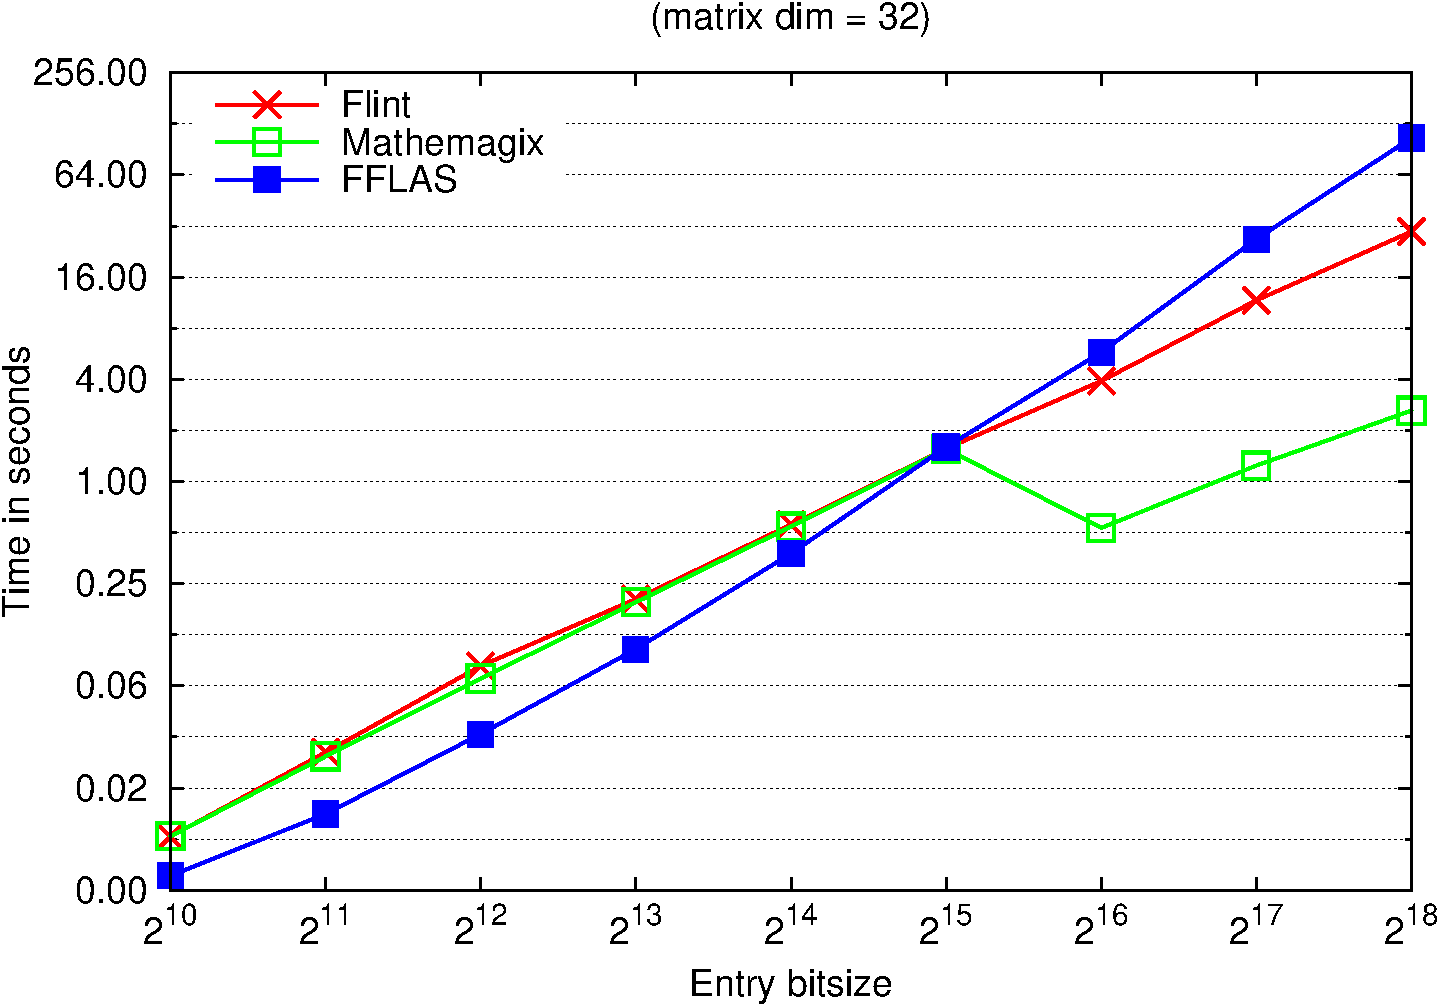
\includegraphics[width = \mywidth]{BENCH/bench-mul-0.pdf}
	}
	\subfloat{
		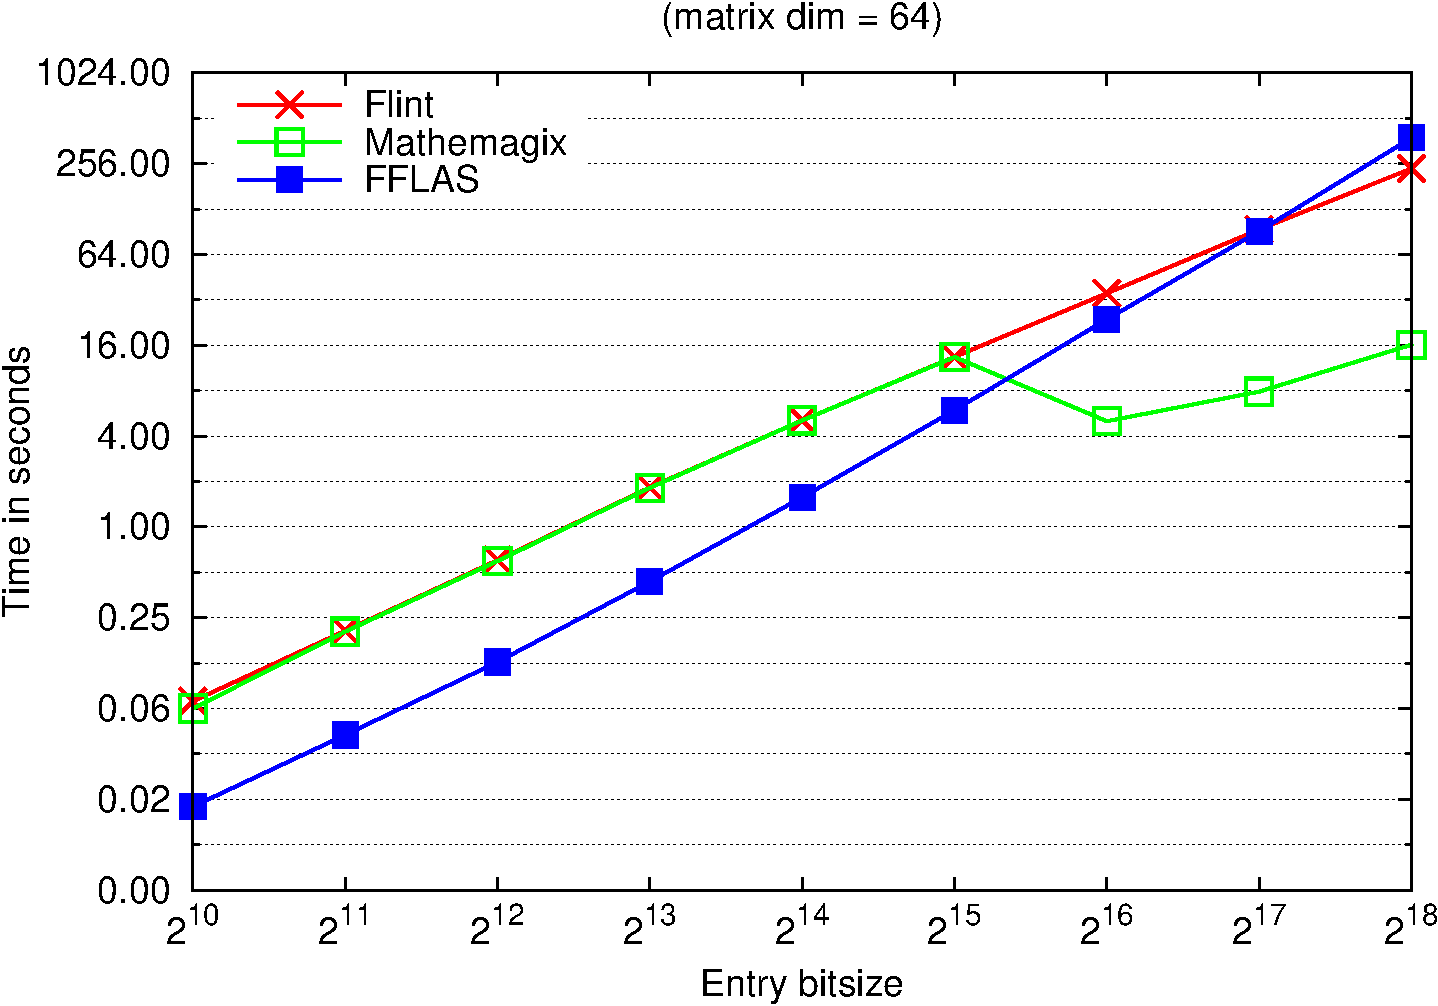
\includegraphics[width = \mywidth]{BENCH/bench-mul-1.pdf}
	}\\
	\subfloat{
		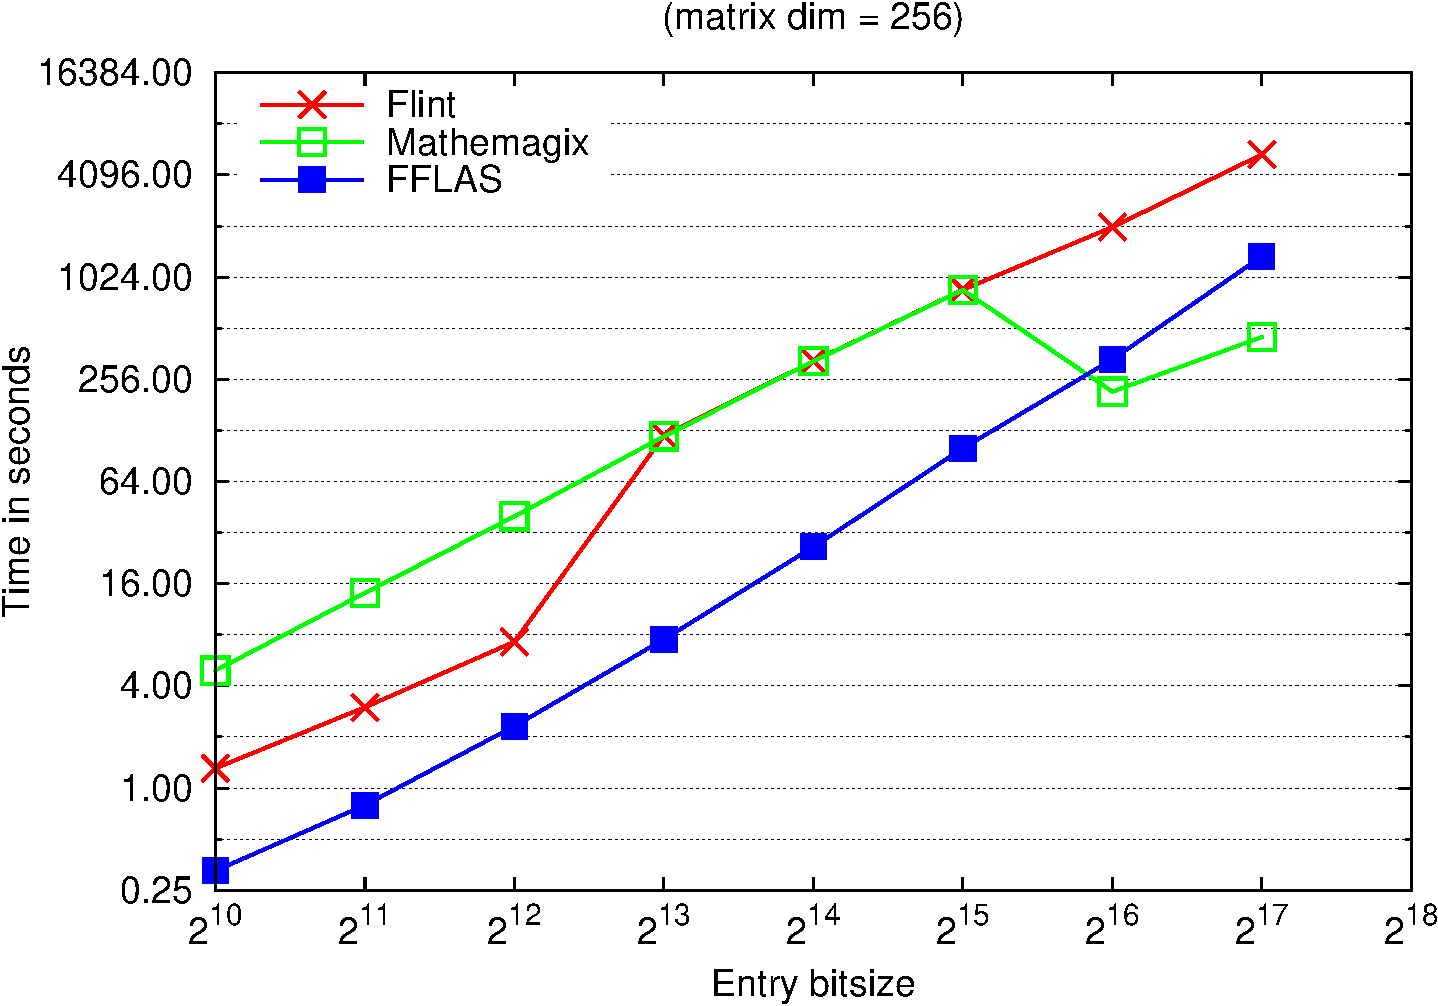
\includegraphics[width = \mywidth]{BENCH/bench-mul-2.pdf}
	}
	\subfloat{
		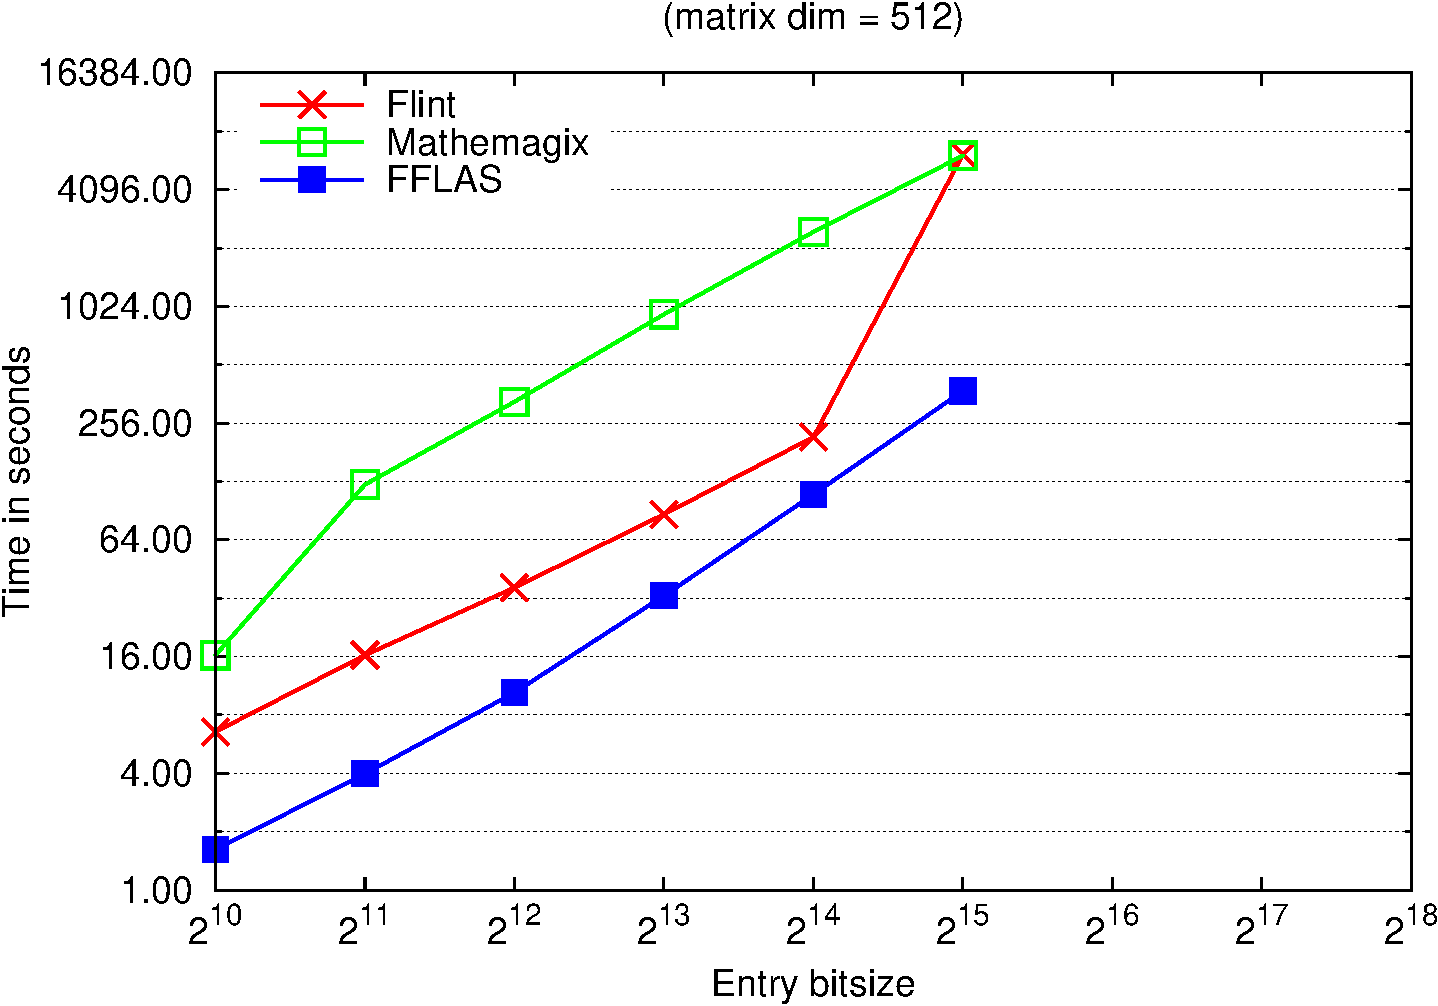
\includegraphics[width = \mywidth]{BENCH/bench-mul-3.pdf}
	}
	\caption{Multi-precision integer matrix multiplication}
	\label{fig:exp-mm}
\end{figure}

Our benchmarks are done on an Intel Xeon E5-2697 2.6 GHz machine. As seen in Figure 
\ref{fig:exp-mm} our linear algebra implementation starts to outperform other implementations as 
the dimensions of the input matrices increase. Due to large entry sizes higher dimensional matrices 
become intractable. For tractable matrices, when the entry sizes are not to large compared to the 
dimension $n$, our algorithm offer very good performances. For example, Table \ref{table:h-dim-mm} 
shows timings for a higher dimension and lower entry sizes.

\begin{table}[ht]
	\renewcommand{\arraystretch}{1.4}
	\tbl{$1024 \times 1204$ integer matrix multiplication
		\label{table:h-dim-mm}}{
	\begin{tabular}{cccc}
		\bf bitsize & \bf FLINT & \bf Mathemagix & \bf FFLAS \\
		\hline
		4096 & 184s & 2536s & 54s \\
		8192 & 427s & 7562s & 156s \\
	\end{tabular}
	}
\end{table}




%////////////////////////////////////////////////


\section{Example Applications}
\label{sec:exapp}

Matrix multiplication is a fundamental operation for many computational problems. In particular, 
integer matrix multiplication comes to play when one deals with finite fields. Prime finite fields, 
denoted by $\F_p$ for a given prime $p$, are usually represented using the set of integers $\{0, 1, 
\dots, p - 1 \}$. Then general finite fields are represented using polynomials over this set of 
integers. In this section, we briefly review some important operations in finite field arithmetic, 
and show how our linear algebra implementations of these operations result in significant speed-ups 
over conventional implementations.

\paragraph{Modular polynomial composition}
Given a field $\F_p$ and polynomials $f, g, h$ of degrees less than $n$ over $\F_p$, modular 
composition is the problem of computing $f(g) \bmod h$. The upper-bound cost of this operations is 
denoted by $\C(n)$ counted as operations over $\F_p$. The well-known algorithm of Brent and Kung 
\cite{BrKu78}, which is implemented by most computer algebra systems, gives the bound $\C(n) = 
O(n^{(\omega+1)/2})$. The bottleneck of their algorithm can be written as a matrix multiplication. 
More precisely, for $k = \lceil \sqrt{n + 1} \rceil$, $f(x) = f_0 + f_1x + \cdots + f_{n - 1}x^{n - 
1}$, and $q(x) = g_0 + g_1x + \cdots + g_{n - 1}x^{n - 1}$ we should compute the matrix 
multiplication
\[
\renewcommand{\arraystretch}{1.5}
\begin{bmatrix}
	f_0^{(0)} & f_0^{(1)} & \cdots & f_0^{(k - 1)} \\
	f_1^{(0)} & f_1^{(1)} & \cdots & f_1^{(k - 1)} \\
	\vdots  & \vdots  & \ddots & \vdots  \\
	f_n^{(0)} & f_n^{(1)} & \cdots & f_n^{(k - 1)}
\end{bmatrix}
\begin{bmatrix}
	g_0 & g_k & \cdots & g_{(k - 1)k} \\
	g_1 & g_{k + 1} & \cdots & g_{(k - 1)k + 1} \\
	\vdots  & \vdots  & \ddots & \vdots  \\
	g_{k - 1} & g_{2k - 1} & \cdots & g_{k^2 - 1}
\end{bmatrix}
\]
where $f_i^{(j)}$ is the $i$-th coefficient of the power $f^j$. We have implemented modular 
polynomials composition using our matrix multiplication in C++. Figure \ref{fig:mod-comp} compares 
our implementation to the \verb|CompMod| method of NTL library \cite{ntl2015} on an Intel(R) 
Core(TM) i7-4790, 3.60GHz machine.

\paragraph{Power projection}
Let $f$ be a polynomial of degree $n$ over $\F_p$, and let $g \in F = \F_p[x] / (f)$. For vectors 
$v, u \in \F_p^n$ denote by $\langle v, u \rangle$ their inner product. Coefficients of polynomials 
over $F$ can be considered as vectors in $\F_p^n$. The power projection problem is computing the 
sequence
\[ \langle v, 1\rangle, \langle v, g\rangle , \dots, \langle v, g^{m - 1} \rangle \]
for a given integer $m > 0$. The best known algorithm for power projection is due to 
\cite{Shoup1999}. The dominant part of the algorithm can be formulated as a matrix multiplication 
similar to the one for modular polynomial composition. Similar to modular composition, we have 
implemented power projection using our matrix multiplication. The implementation is in C++ on an 
Intel(R) Core(TM) i7-4790, 3.60GHz machine. Figure \ref{fig:power-proj} compares implementation to 
the \verb|ProjectPowers| method of NTL. 

\begin{figure}[ht]
	\def\mywidth{6.5cm}
	\subfloat[Modular polynomial composition]{
		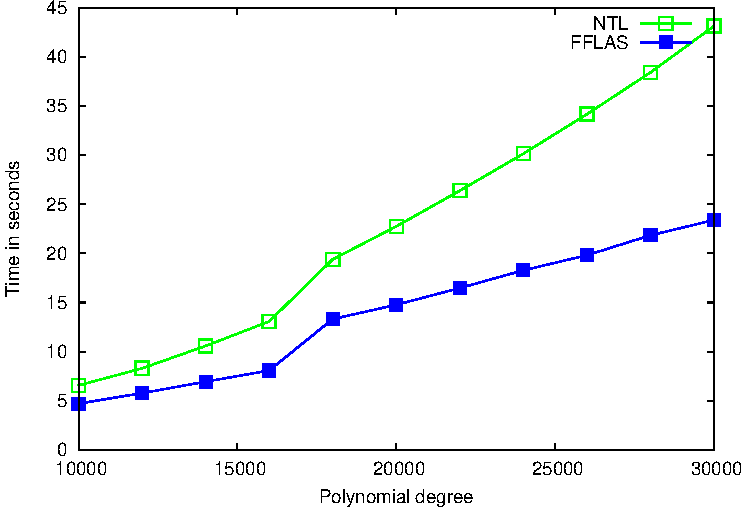
\includegraphics[width = \mywidth]{BENCH/mod-comp/mod-comp.pdf}
		\label{fig:mod-comp}
	}
	\subfloat[Power projection]{
		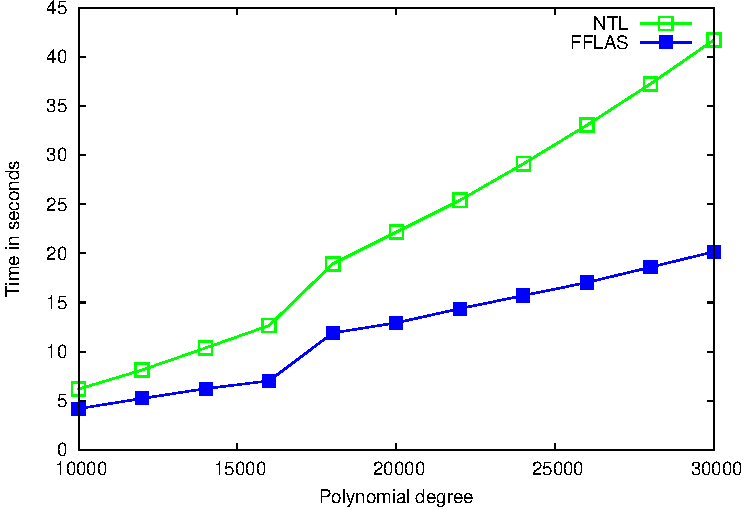
\includegraphics[width = \mywidth]{BENCH/mod-comp/power-proj.pdf}
		\label{fig:power-proj}
	}
\end{figure}

The above two operations are main ingredients of many higher level operations in finite fields. Two 
such operations are \textit{Minimal polynomial computation}, and \textit{Polynomial factorization}. 
Let $f \in \F_p[X]$ be a polynomial of degree $n$, and let $a \in \F_p[X] / (f)$. The minimal 
polynomial of $a$ over $\F_p$ is a monic irreducible polynomial $g \in F_p[X]$ of degree less than 
$n$ such that $g(a) = 0 \bmod f$. An efficient algorithm for computing minimal polynomials is 
presented in \cite{Shoup1999}, which uses power projection.

Given $f \in \F_p[X]$, polynomial factorization is the problem of expressing $f$ as a product of 
irreducible factors. A well-known algorithm for factoring polynomials is due to 
\cite{Cantor1981}. One of the main operations in the algorithm is modular polynomial composition, 
as explained in \cite{von1992}. We have modified the minimal polynomial and factoring 
implementations in NTL to use our new power projection and modular composition. Figures 
\ref{fig:min-poly}, \ref{fig:factoring} compare the methods \verb|MinPolyMod| and \verb|CanZass| of 
NTL to their new versions on an Intel(R) Core(TM) i7-4790, 3.60GHz machine.

\begin{figure}[ht]
	\def\mywidth{6.5cm}
	\subfloat[Minimal polynomial computaion]{
		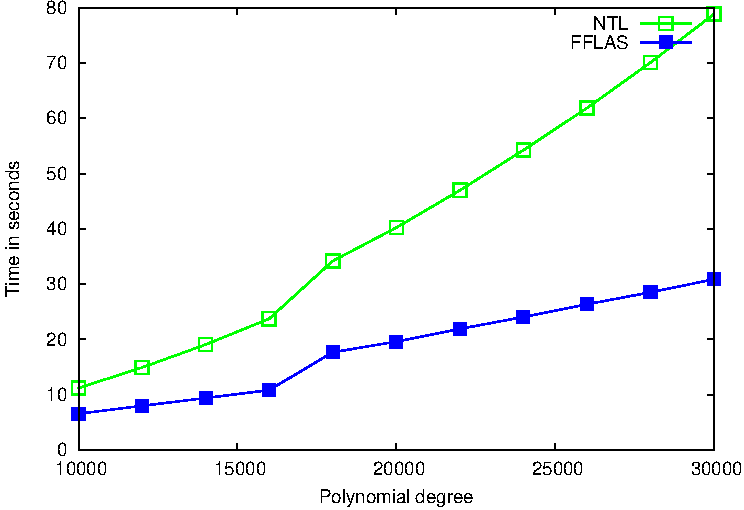
\includegraphics[width = \mywidth]{BENCH/mod-comp/min-poly.pdf}
		\label{fig:min-poly}
	}
	\subfloat[Polynomial factorization]{
		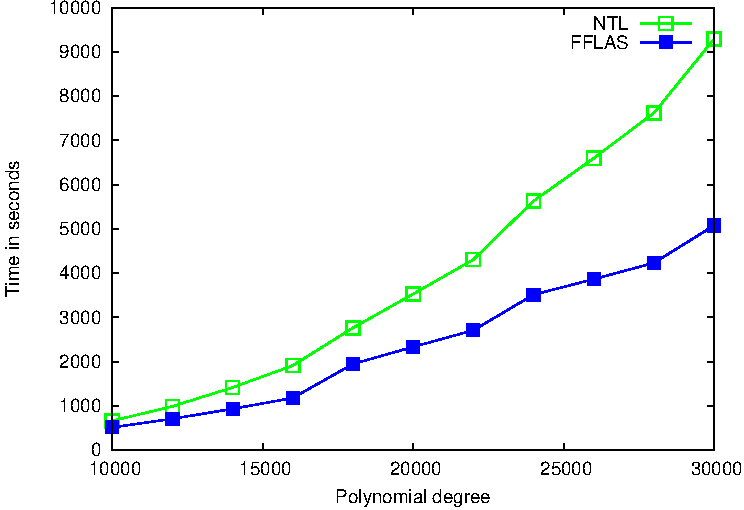
\includegraphics[width = \mywidth]{BENCH/mod-comp/factoring.pdf}
		\label{fig:factoring}
	}
\end{figure}















%{\color{red}
%All the codes are available in the FFLAS\_FFPACK Library (see 
%https://github.com/linbox-team/fflas-ffpack).
%\begin{itemize}
%\item The simultaneous reduction/reconstruction's code is available in the file:\\ 
%\texttt{fflas-ffpack/fflas-ffpack/field/rns-double.inl}
%\item The matrix multiplication code is available in the file: 
%\\\texttt{fflas-ffpack/fflas-ffpack/fflas/fflas\_fgemm/fgemm\_classical\_mp.inl}
%\end{itemize}
%}
%\subsection{Reduction to word-size matrix multiplication}
%how to store intermediate matrices (Kronecker matrix) in order to optimize cache
%efficiency (transpose is delayed to the matrix multiplication). We always want
%the Kronecker matrix to be stored $\beta$-adic major.  How to choose $\beta$ and
%the $m_i$ to guarantee the result to fit into a word-size register.
%
%\subsection{Kronecker substitution}
%$\beta$ is chosen to be $2^{16}$ in order to do not require any arithmetic
%operation.  Can we do better with a larger beta ? What is the compromise between
%$\beta$ and the $m_i$ ?
%
%Reconstruction from the almost $\beta$-adic to GMP integer using a splitting of
%the $beta$-adic expansion into four GMP integer. ? Can we do better do reduce the
%result mod $\prod m_i$.
%
%\subsubsection{From integer to $\beta$-adic}
%using gmp structure we can do this for free. only cast mpz data to uint16.
%
%\subsection{Linear storage for multi-modular matrix}
%explication lda, rda , RNSMajor ou MatrixMajor
%\section{Benchmarks}


\bibliographystyle{ACM-Reference-Format-Journals}
\bibliography{biblio}
\end{document}
  
